\documentclass{article}
\documentclass{article}


    \usepackage[utf8]{inputenc}
    \usepackage[english]{babel}
    \usepackage{blindtext}
    \usepackage{cancel}
    \usepackage{hyperref}
    \usepackage{amssymb,amsmath,amsthm}
    \usepackage{mdframed}
    \usepackage{systeme,mathtools}
    \usepackage{array}
    \usepackage{multirow}
    \usepackage{tabu}
    \usepackage{fancyhdr}
    \usepackage[english]{babel}
    
    \usepackage[
     width=210mm,
     height=297mm,
     lmargin= 35mm,
     rmargin= 30mm,
     bmargin=25mm,
     tmargin=25mm,
     textwidth=165mm,
     textheight=110mm,
     ]{geometry}
     \usepackage{graphicx}
    

\begin{document}

\pagenumbering{arabic}

\newpage

\tableofcontents

\newpage
\section{Tipologia Esercizio 1}
In particolare verranno trattati gli esercizi riguardanti:
\begin{itemize}
\item Caduta di un corpo da fermo
\item Moto proiettile
\item Moto Circolare Uniforme
\end{itemize}
\begin{figure}[h!]
\textbf{Tema d'Esame di Gennaio 2015}\\ \\
Si determini la differenza di potenziali ai capi della resistenza $R4$ del circuito mostrato in figura. La differenza di potenziale fornita dalla batteria è di $12V$ e i valori delle resistenze sono rispettivamente $R2=15\Omega, R3=40\Omega, R4=25\Omega, R5=R6=32\Omega, R1=R7=18\Omega$
\begin{center}
		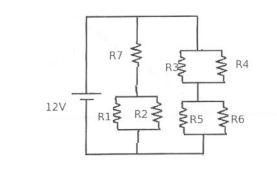
\includegraphics[scale=1.2]{ES5/GEN052015.jpg}
	\end{center}
	\begin{boxed}
		\null\hfill \textbf{Soluzione:} $V_4 = 5.85 V$\\
		\textbf{Procedimento: } \\
		Semplificazione delle Resistenze:\\
		$R_{34}=\frac{R_3\cdot R_4}{R_3+R_4}=\frac{40\Omega \cdot 25\Omega}{40\Omega+25\Omega}=15.38\Omega$\\
		$R_{56}=\frac{R_5\cdot R_6}{R_5+R_6}=\frac{32\Omega \cdot 32\Omega}{32\Omega+32\Omega}=16\Omega$\\
		$R_{12}=\frac{R_1\cdot R_2}{R_1+R_2}=\frac{18\Omega \cdot 15\Omega}{18\Omega+15\Omega}=8.18\Omega$\\
		$R_{127}=R_{12}+R_7=8.18\Omega + 18\Omega=26.18\Omega$\\
		$R_{3456}=R_{34}+R_{56}=15.38\Omega+16\Omega=31.38\Omega$\\
		$R_{tot}=\frac{R_{127}\cdot R_{3456}}{R_{127}+R_{3456}}=\frac{26.18\Omega \cdot 31.38\Omega}{26.18\Omega + 31.38\Omega}=14.23\Omega$\\
		Ricordando che la Tensione in parallelo non cambia, così come non cambia la corrente in serie:\\
		$V_{tot}=V_{127}=V_{3456}=12V$\\
		$I_{3456}=\frac{V_{3456}}{R_{3456}}=0.38A \qquad I_{3456}=I_{34}=I_{56}$\\
		$V_{34}=V_3=V_4=R_{34}\cdot I_{34}=15.38\Omega \cdot 0.38A=5.85\Omega \qquad V_{34}=V_3=V_4$
	\end{boxed}
\end{figure}

\begin{figure}[h!]
\textbf{Tema d'Esame di Febbraio 2015}\\ \\
 Nel circuito in figura, la corrente attraverso $R6$ è $i_6=1.40A$ e le resistenze sono
$R1=R2=R3=2.0\Omega, R4= 16.0\Omega, R5= 8.0 \Omega e R6= 4.0 \Omega$. Qual'è la forza elettromotrice della batteria (ideale)?
\begin{center}
		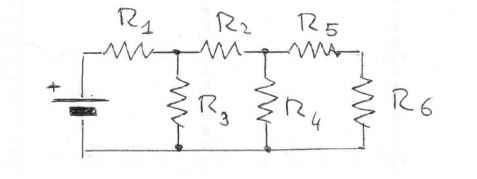
\includegraphics[scale=0.8]{ES5/FEB052015.jpg}
	\end{center}
\end{figure}

\begin{figure}[h!]
\textbf{Tema d'Esame di Giugno 2015}\\ \\
Si determini la differenza di potenziali ai capi della resistenza R4 del circuito mostrato in figura. La differenza di potenziale fornita dalla batteria è di $12V$ e i valori delle resistenze sono rispettivamente $R2=15\Omega, R3=40\Omega, R4=25\Omega, R5=R6=32\Omega, R1=R7=18\Omega$.
\begin{center}
		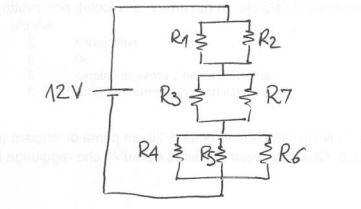
\includegraphics[scale=1]{ES5/GIU052015.jpg}
	\end{center}
\end{figure}

\begin{figure}[h!]
\textbf{Tema d'Esame di Luglio 2015}\\ \\
La differenza di potenziale fornita dalla batteria è di $12V$ e i valori delle resistenze sono rispettivamente $R2=15\Omega, R3=40\Omega, R4=25\Omega, R5=R6=32\Omega, R1=R7=18\Omega$
\begin{center}
		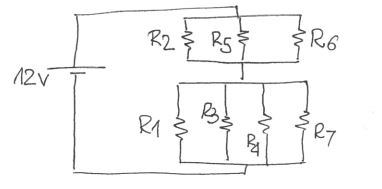
\includegraphics[scale=1]{ES5/LUG052015.jpg}
	\end{center}
\end{figure}

\begin{figure}[h!]
    \textbf{Tema d'Esame di Gennaio 2016}\\ \\
    Una molla viene compressa di 17 cm prima di lanciare una palla verso un piano inclinato
    senza attrito. La palla ha massa 1kg e il piano inclinato ha un'altezza H=1.28 m. Quanto vale
    la costante elastica della molla affinché la palla arrivi con una velocità di 4 m/s in cima al
    piano ?
    \\
        \begin{center}
            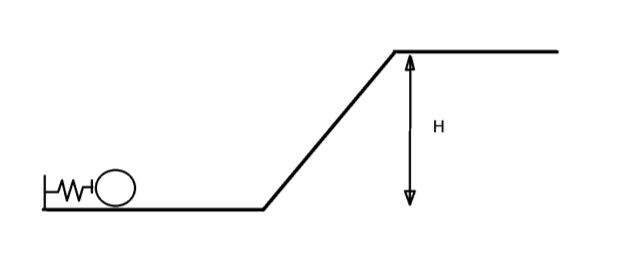
\includegraphics[scale=0.5]{ES2/GEN022016.jpg}
        \end{center}
    \end{figure}
    
    \begin{figure}[h!]
    \textbf{Tema d'Esame di Febbraio 2016}\\ \\
    Una palla di massa $250g$ è lanciata da una molla con costante elastica $63 N/m$ compressa di $45 cm$. La palla viaggia attraverso un piano inclinato alto $72 cm$. Una volta arrivata in cima al piano inclinato la palla incontra una superficie piatta frenante. Il coefficente d'attrito dinamico palla-superficie è di $m=0.42$. Che distanza percorre la palla sulla superficie frenante prima di fermarsi?
    \\
        \begin{center}
            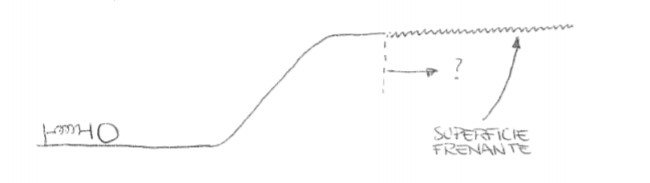
\includegraphics[scale=0.5]{ES2/FEB022016.jpg}
        \end{center}
        \noindent\fbox{
            \parbox{\textwidth}{
                \null\hfill \textbf{Soluzione:} $ s=4.477m $\\
                \textbf{Procedimento: } \\
                Trasformare le unità di misura:\\
                $\Delta x= 45cm =0.45m$\\
                $h=72cm=0.72m$\\ \\
                Impostando il seguente sistema, considerando come punto A la molla , il punto B il punto immediatamente dopo il piano inclinato e il punto C dove la palla si fermerà sul piano scabro.\\
                $$
                \begin{cases}
                    U_{El,A} = U_B + K_B \\
                    U_B + K_B = U_C + L_a
                \end{cases}
                =
                \begin{cases}
                    \frac{1}{2}\cdot k \cdot \Delta x^2 = m\cdot g \cdot h + \frac{1}{2} \cdot m \cdot v^2\\
                    \frac{1}{2}\cdot m \cdot v^2 = \mu_d \cdot m \cdot g \cdot cos(\alpha) \cdot \Delta s
                \end{cases}
                $$
                $$
                \begin{cases}
                    6.378J = 1.766J + 0.125kg \cdot v^2\\
                    0.125kg\cdot v^2 = 103N \cdot \Delta s
                \end{cases}
                =
                \begin{cases}
                    v^2 = 36.896 m^2/s^2 \\
                    \Delta s= 4.477m
                \end{cases}
                $$
                
            }
        }                  
    \end{figure}
    
    \begin{figure}[h!]
    \textbf{Tema d'Esame di Giugno 2016}\\ \\
    Una molla ideale può essere compressa di $1.0 m$ da una forza di $100 N$. La stessa molla è posta alla fine di un piano inclinato con attrito (coefficiente $0.2$) che forma un angolo di 30$^{\circ}$ con l'orizzontale. Una massa $M$ di $10 kg$ viene lasciata cadere da ferma dal vertice del piano inclinato e si arresta momentaneamente dopo aver compresso la molla di $2.0 m$. Qual'è la velocità della massa un attimo prima di toccare la molla? 
    \\
        \begin{center}
            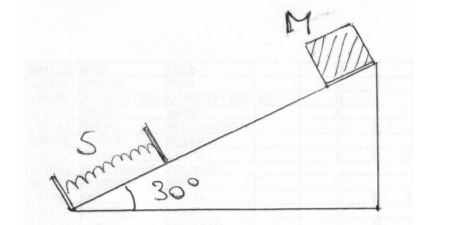
\includegraphics[scale=0.5]{ES2/GIU022016.jpg}
        \end{center}

        \noindent\fbox{
            \parbox{\textwidth}{
                \null\hfill \textbf{Soluzione:} $ s=6.324m/s $\\
                \textbf{Procedimento: } \\
                Trasformare le unità di misura:\\
                $\Delta x= 45cm =0.45m$\\
                $h=72cm=0.72m$\\ \\
                Impostando il seguente sistema, considerando come punto A la molla , il punto B dove parte il corpo.\\
                È conveniente ribaltare la struttura del problema per dire che la massa parte dalla molla e arriva nel punto B con velocità 0.\\
                $$
                \begin{cases}
                    U_{El,A} - L_a= U_B  \\
                    K_A - L_a = U_B
                \end{cases}
                =
                \begin{cases}
                    \frac{1}{2}\cdot k \cdot \Delta x^2 - \mu_d \cdot m \cdot g \cdot cos(\alpha) \cdot \Delta s= m\cdot g \cdot h \\
                    \frac{1}{2}\cdot m \cdot v^2 - \mu_d \cdot m \cdot g \cdot cos(\alpha) \cdot \Delta s=m\cdot g \cdot h
                \end{cases}
                $$
                Nota: con la seconda equazione del sistema ipotizziamo che a prescindere che sia stata spinta da una molla, calcoliamo la velocità necessaria che serve per spingere un corpo su una superficie scabra. \\
                A questo punto basta solamente eguagliare:\\
                $\frac{1}{2}\cdot k \cdot \Delta x^2 = \frac{1}{2}\cdot m \cdot v^2 \quad 200J=5kg\cdot v^2 \quad v=\sqrt{40m^2 /s^2}=6.324m/s$\\

               
                
            }
        }    
    \end{figure}
    
    \begin{figure}[h!]
    \textbf{Tema d'Esame di Luglio 2016}\\ \\
    La molla della figura ha una costante elastica $k = 120 \frac{N}{m}$ e una lunghezza a riposo di $45cm$. Quando un blocco di massa $M$ viene attaccato alla molla l'estensione di equilibrio della molla è $60cm$. Il piano inclinato è liscio(senza attrito) e forma un angolo di $40^\circ$ con l'orizzontale. Se la massa viene tirata leggermente verso il basso e viene rilasciata, qual è il periodo di oscillazione? 
    \\
        \begin{center}
            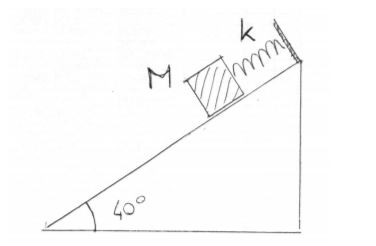
\includegraphics[scale=0.5]{ES2/LUG022016.jpg}
        \end{center}
    \end{figure}
    
    
\begin{figure}[h!]
\textbf{Tema d'Esame di Febbraio 2017}\\ \\
Sapendo che la resistenza $R8$ è attraversata da una corrente $i_8 = 0.20 A$, si calcoli la corrente che attraversa $R3$. Si considerino le seguenti resistenze $R8 = 10 \Omega, R1 = R2 = R3 = 5.0 \Omega , R4 = 12 \Omega , R5 = 15 \Omega $.
	\begin{center}
		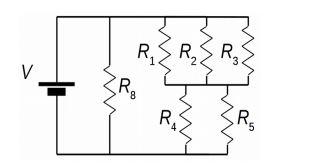
\includegraphics[scale=1.1]{ES5/FEB052017.jpg}
	\end{center}
	\noindent\fbox{
		\parbox{\textwidth}{
			\null\hfill \textbf{Soluzione:} $I_3 = 0.08A$\\
			\textbf{Procedimento: } \\
			Semplificazione delle Resistenze:\\
			$R_{123}=\frac{1}{\frac{1}{R_1}+\frac{1}{R_2}+\frac{1}{R_3}}=\frac{1}{\frac{1}{5\Omega}+\frac{1}{5\Omega}+\frac{1}{5\Omega}}=1.67\Omega$\\ \\ 
			$R_{45}=\frac{R_4\cdot R_5}{R_4 + R_5}=\frac{12\Omega\cdot 15\Omega}{12\Omega + 15\Omega}=6.67\Omega$\\
			$R_{12345}=R_{123}+R_{45}=6.67\Omega+1.67\Omega=8.34\Omega$\\
			Ricordando che la tensione in parallelo non cambia, così come non cambia la corrente in serie:\\
			$V_{tot}=V_{12345}=V_8=R_8\cdot I_8=10\Omega\cdot 0.2A=2V$\\
			$I_{12345}=I_{123}=I_{45}=\frac{V}{R_{12345}}=\frac{2V}{8.34\Omega}=0.24A$\\
			$V_{123}=R_{123}\cdot I_{12345}=1.67\Omega\cdot 0.24A=0.40V$\\
			$I_3=\frac{V_{123}}{R_3}=\frac{0.40V}{5\Omega}=0.08A$
		}
	}	
	
\end{figure}

\begin{figure}[h!]
\textbf{Tema d'Esame di Giugno 2017}\\ \\
 Si determini il valore della resistenza $R_x$ del circuito mostrato nella figura sotto a sinistra. La differenza di potenziale fornita dalla batteria è $3 V$, la corrente $i_3$ che scorre nella resistenza $R_3$ è pari a $0.1 A$ ed i valori delle altre resistenze nel circuito
sono $R1 = R2 = 5 \Omega ,R3 = R4 = 10 \Omega$.
	\begin{center}
		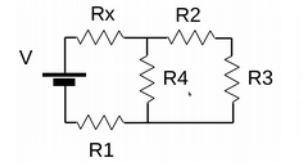
\includegraphics[scale=1.1]{ES5/GIU052017.jpg}
	\end{center}
	\noindent\fbox{
		\parbox{\textwidth}{
			\null\hfill \textbf{Soluzione:} $R_x = 1\Omega$\\
			\textbf{Procedimento: } \\
			Ricordando che la tensione in parallelo non cambia, così come non cambia la corrente in serie proseguiamo semplificando le resistenze e aggiornando man mano corrente e tensione:\\
			
			
			$R_{23}=R_2 + R_3=5\Omega + 10\Omega=15\Omega$\\
			$I_3=I_2=I_{23}=0.1A$\\
			$V_{23}=V_{234}=V_4=R_{23} \cdot I_{23}=15\Omega \cdot 0.1A=1.5V$\\
			$I_{234}=\frac{V_{234}}{R_{234}}=\frac{1.5V}{6\Omega}=0.25A$\\
			$V_1=R_1\cdot I_{234}=5\Omega \cdot 0.25A=1.25V$\\
			$V_x=V_{tot}- V_1 - V_{234}=3V - 1.25V -1.5V=0.25V$\\
			$R_x=\frac{V_x}{I_{234}}=\frac{0.25V}{0.25A}=1\Omega$
		}
	}	
\end{figure}

\begin{figure}[h!]
\textbf{Tema d'Esame di Settembre 2017}\\ \\
Trovare le correnti $i_1, i_2 , i_3$ nei tre rami del circuito qui sotto.
$R1 = 4.0 \Omega, R2 = 6.0 \Omega, R3 = 3.0 \Omega$ ed $ E 1 = 1.5 V,  E 2 = 3.0 V$.
	\begin{center}
		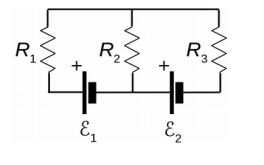
\includegraphics[scale=1.1]{ES5/SET052017.jpg}
	\end{center}
	\noindent\fbox{
		\parbox{\textwidth}{
			\null\hfill \textbf{Soluzione:} $R_x = 1\Omega$\\
			\textbf{Procedimento: } \\
			In questa tipologia di esercizio si deve impostare il sistema per poi trovare le rispettive correnti, per farlo bisogno stabilire arbitrariamente il verso della corrente di ogni maglia.\\
			 Nel nostro caso supporremo che la corrente viaggi in senso orario in entrambe le maglie.\\

			\systeme*{
				I_1=I_2 +I_3,
				\varepsilon_1= R_1\cdot I_1 + R_2\cdot I_2,
				\varepsilon_2= -R_2\cdot I_2 + R_3\cdot I_3
			}
			\\ \\
			Risolvendo il sistema si otterranno i valori delle correnti.\\ \\
			\systeme*{
				I_1=I_2 +I_3,
				1.5= 4\cdot I_1 + 6\cdot I_2,
				3= -6\cdot I_2 + 3\cdot I_3
			}
			\hspace{1.45cm} = \hspace{1.5cm}
			\systeme*{
				I_1=I_2 +I_3,
				1.5= 4\cdot I_2 + 4\cdot I_3 + 6\cdot I_2,
				3= -6\cdot I_2 + 3\cdot I_3
			}\\ \\
			\systeme*{
				I_1=I_2 +I_3,
				1.5= 10\cdot I_2 + 4\cdot I_3,
				I_3=\frac{3V +6\cdot I_2}{3}
			}
			\hspace{1.5cm} = \hspace{1.5cm}
			\systeme*{
				I_1=I_2 +I_3,
				1.5= 10\cdot I_2 + 4\cdot (1 +2\cdot I_2),
				3= -6\cdot I_2 + 3\cdot I_3
			}\\ \\
			\systeme*{
				I_1=I_2 +I_3,
				I_2= -0.139,
				I_3= 1 +2\cdot I_2
			}
			\hspace{2.45cm} = \hspace{1.45cm}
			\systeme*{
				I_1=-0.139 +I_3,
				I_2= -0.139,
				I_3= 0.722
			}\\ \\
			\systeme*{
				I_1= 0.583A,
				I_2= -0.139A,
				I_3= 0.722A
			}\\ \\
		}
	}	
	
\end{figure}
\begin{figure}[h!]
\textbf{Tema d'Esame di Gennaio 2018}\\ \\
Una persona di massa $70.0 kg$ sta su una bilancia posta all’equatore sulla
superficie di un pianeta (supposto perfettamente sferico e uniforme). Qual è il
peso misurato dalla bilancia se il diametro del pianeta è il doppio di quello della
terra, ma la sua densità media ed il suo periodo di rotazione sono gli stessi della
terra? ($M_T = 5.97\cdot 10^{24}kg, R_T = 6370 km, T_T = 24.0 h$) 
\end{figure}

\clearpage
\newpage
\section{Tipologia Esercizio 2}
In particolare verranno trattati gli esercizi riguardanti:
\begin{itemize}
\item Piano Inclinato 
\end{itemize}

\begin{figure}[h!]
    \textbf{Tema d'Esame di Gennaio 2016}\\ \\
    Una molla viene compressa di 17 cm prima di lanciare una palla verso un piano inclinato
    senza attrito. La palla ha massa 1kg e il piano inclinato ha un'altezza H=1.28 m. Quanto vale
    la costante elastica della molla affinché la palla arrivi con una velocità di 4 m/s in cima al
    piano ?
    \\
        \begin{center}
            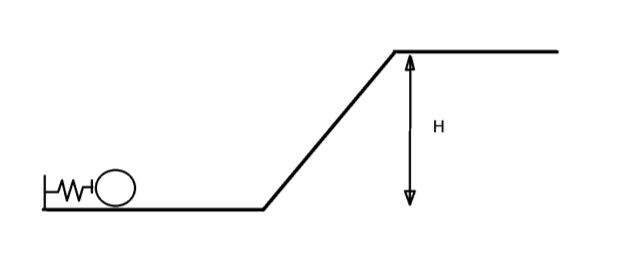
\includegraphics[scale=0.5]{ES2/GEN022016.jpg}
        \end{center}
    \end{figure}
    
    \begin{figure}[h!]
    \textbf{Tema d'Esame di Febbraio 2016}\\ \\
    Una palla di massa $250g$ è lanciata da una molla con costante elastica $63 N/m$ compressa di $45 cm$. La palla viaggia attraverso un piano inclinato alto $72 cm$. Una volta arrivata in cima al piano inclinato la palla incontra una superficie piatta frenante. Il coefficente d'attrito dinamico palla-superficie è di $m=0.42$. Che distanza percorre la palla sulla superficie frenante prima di fermarsi?
    \\
        \begin{center}
            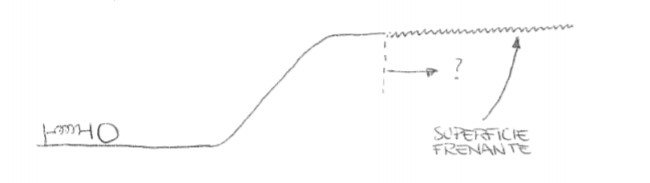
\includegraphics[scale=0.5]{ES2/FEB022016.jpg}
        \end{center}
        \noindent\fbox{
            \parbox{\textwidth}{
                \null\hfill \textbf{Soluzione:} $ s=4.477m $\\
                \textbf{Procedimento: } \\
                Trasformare le unità di misura:\\
                $\Delta x= 45cm =0.45m$\\
                $h=72cm=0.72m$\\ \\
                Impostando il seguente sistema, considerando come punto A la molla , il punto B il punto immediatamente dopo il piano inclinato e il punto C dove la palla si fermerà sul piano scabro.\\
                $$
                \begin{cases}
                    U_{El,A} = U_B + K_B \\
                    U_B + K_B = U_C + L_a
                \end{cases}
                =
                \begin{cases}
                    \frac{1}{2}\cdot k \cdot \Delta x^2 = m\cdot g \cdot h + \frac{1}{2} \cdot m \cdot v^2\\
                    \frac{1}{2}\cdot m \cdot v^2 = \mu_d \cdot m \cdot g \cdot cos(\alpha) \cdot \Delta s
                \end{cases}
                $$
                $$
                \begin{cases}
                    6.378J = 1.766J + 0.125kg \cdot v^2\\
                    0.125kg\cdot v^2 = 103N \cdot \Delta s
                \end{cases}
                =
                \begin{cases}
                    v^2 = 36.896 m^2/s^2 \\
                    \Delta s= 4.477m
                \end{cases}
                $$
                
            }
        }                  
    \end{figure}
    
    \begin{figure}[h!]
    \textbf{Tema d'Esame di Giugno 2016}\\ \\
    Una molla ideale può essere compressa di $1.0 m$ da una forza di $100 N$. La stessa molla è posta alla fine di un piano inclinato con attrito (coefficiente $0.2$) che forma un angolo di 30$^{\circ}$ con l'orizzontale. Una massa $M$ di $10 kg$ viene lasciata cadere da ferma dal vertice del piano inclinato e si arresta momentaneamente dopo aver compresso la molla di $2.0 m$. Qual'è la velocità della massa un attimo prima di toccare la molla? 
    \\
        \begin{center}
            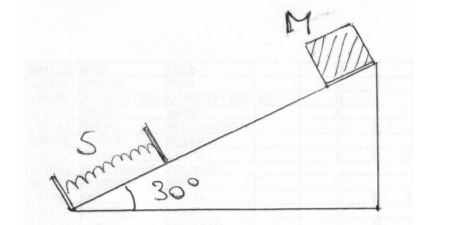
\includegraphics[scale=0.5]{ES2/GIU022016.jpg}
        \end{center}

        \noindent\fbox{
            \parbox{\textwidth}{
                \null\hfill \textbf{Soluzione:} $ s=6.324m/s $\\
                \textbf{Procedimento: } \\
                Trasformare le unità di misura:\\
                $\Delta x= 45cm =0.45m$\\
                $h=72cm=0.72m$\\ \\
                Impostando il seguente sistema, considerando come punto A la molla , il punto B dove parte il corpo.\\
                È conveniente ribaltare la struttura del problema per dire che la massa parte dalla molla e arriva nel punto B con velocità 0.\\
                $$
                \begin{cases}
                    U_{El,A} - L_a= U_B  \\
                    K_A - L_a = U_B
                \end{cases}
                =
                \begin{cases}
                    \frac{1}{2}\cdot k \cdot \Delta x^2 - \mu_d \cdot m \cdot g \cdot cos(\alpha) \cdot \Delta s= m\cdot g \cdot h \\
                    \frac{1}{2}\cdot m \cdot v^2 - \mu_d \cdot m \cdot g \cdot cos(\alpha) \cdot \Delta s=m\cdot g \cdot h
                \end{cases}
                $$
                Nota: con la seconda equazione del sistema ipotizziamo che a prescindere che sia stata spinta da una molla, calcoliamo la velocità necessaria che serve per spingere un corpo su una superficie scabra. \\
                A questo punto basta solamente eguagliare:\\
                $\frac{1}{2}\cdot k \cdot \Delta x^2 = \frac{1}{2}\cdot m \cdot v^2 \quad 200J=5kg\cdot v^2 \quad v=\sqrt{40m^2 /s^2}=6.324m/s$\\

               
                
            }
        }    
    \end{figure}
    
    \begin{figure}[h!]
    \textbf{Tema d'Esame di Luglio 2016}\\ \\
    La molla della figura ha una costante elastica $k = 120 \frac{N}{m}$ e una lunghezza a riposo di $45cm$. Quando un blocco di massa $M$ viene attaccato alla molla l'estensione di equilibrio della molla è $60cm$. Il piano inclinato è liscio(senza attrito) e forma un angolo di $40^\circ$ con l'orizzontale. Se la massa viene tirata leggermente verso il basso e viene rilasciata, qual è il periodo di oscillazione? 
    \\
        \begin{center}
            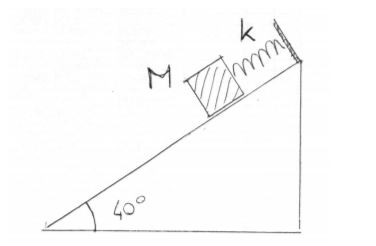
\includegraphics[scale=0.5]{ES2/LUG022016.jpg}
        \end{center}
    \end{figure}
    
    
\begin{figure}[h!]
\textbf{Tema d'Esame di Febbraio 2017}\\ \\
Sapendo che la resistenza $R8$ è attraversata da una corrente $i_8 = 0.20 A$, si calcoli la corrente che attraversa $R3$. Si considerino le seguenti resistenze $R8 = 10 \Omega, R1 = R2 = R3 = 5.0 \Omega , R4 = 12 \Omega , R5 = 15 \Omega $.
	\begin{center}
		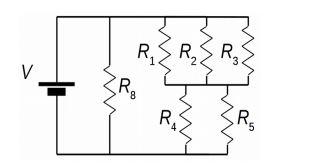
\includegraphics[scale=1.1]{ES5/FEB052017.jpg}
	\end{center}
	\noindent\fbox{
		\parbox{\textwidth}{
			\null\hfill \textbf{Soluzione:} $I_3 = 0.08A$\\
			\textbf{Procedimento: } \\
			Semplificazione delle Resistenze:\\
			$R_{123}=\frac{1}{\frac{1}{R_1}+\frac{1}{R_2}+\frac{1}{R_3}}=\frac{1}{\frac{1}{5\Omega}+\frac{1}{5\Omega}+\frac{1}{5\Omega}}=1.67\Omega$\\ \\ 
			$R_{45}=\frac{R_4\cdot R_5}{R_4 + R_5}=\frac{12\Omega\cdot 15\Omega}{12\Omega + 15\Omega}=6.67\Omega$\\
			$R_{12345}=R_{123}+R_{45}=6.67\Omega+1.67\Omega=8.34\Omega$\\
			Ricordando che la tensione in parallelo non cambia, così come non cambia la corrente in serie:\\
			$V_{tot}=V_{12345}=V_8=R_8\cdot I_8=10\Omega\cdot 0.2A=2V$\\
			$I_{12345}=I_{123}=I_{45}=\frac{V}{R_{12345}}=\frac{2V}{8.34\Omega}=0.24A$\\
			$V_{123}=R_{123}\cdot I_{12345}=1.67\Omega\cdot 0.24A=0.40V$\\
			$I_3=\frac{V_{123}}{R_3}=\frac{0.40V}{5\Omega}=0.08A$
		}
	}	
	
\end{figure}

\begin{figure}[h!]
\textbf{Tema d'Esame di Giugno 2017}\\ \\
 Si determini il valore della resistenza $R_x$ del circuito mostrato nella figura sotto a sinistra. La differenza di potenziale fornita dalla batteria è $3 V$, la corrente $i_3$ che scorre nella resistenza $R_3$ è pari a $0.1 A$ ed i valori delle altre resistenze nel circuito
sono $R1 = R2 = 5 \Omega ,R3 = R4 = 10 \Omega$.
	\begin{center}
		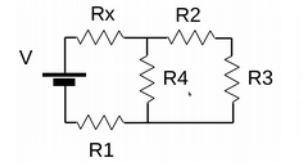
\includegraphics[scale=1.1]{ES5/GIU052017.jpg}
	\end{center}
	\noindent\fbox{
		\parbox{\textwidth}{
			\null\hfill \textbf{Soluzione:} $R_x = 1\Omega$\\
			\textbf{Procedimento: } \\
			Ricordando che la tensione in parallelo non cambia, così come non cambia la corrente in serie proseguiamo semplificando le resistenze e aggiornando man mano corrente e tensione:\\
			
			
			$R_{23}=R_2 + R_3=5\Omega + 10\Omega=15\Omega$\\
			$I_3=I_2=I_{23}=0.1A$\\
			$V_{23}=V_{234}=V_4=R_{23} \cdot I_{23}=15\Omega \cdot 0.1A=1.5V$\\
			$I_{234}=\frac{V_{234}}{R_{234}}=\frac{1.5V}{6\Omega}=0.25A$\\
			$V_1=R_1\cdot I_{234}=5\Omega \cdot 0.25A=1.25V$\\
			$V_x=V_{tot}- V_1 - V_{234}=3V - 1.25V -1.5V=0.25V$\\
			$R_x=\frac{V_x}{I_{234}}=\frac{0.25V}{0.25A}=1\Omega$
		}
	}	
\end{figure}

\begin{figure}[h!]
\textbf{Tema d'Esame di Settembre 2017}\\ \\
Trovare le correnti $i_1, i_2 , i_3$ nei tre rami del circuito qui sotto.
$R1 = 4.0 \Omega, R2 = 6.0 \Omega, R3 = 3.0 \Omega$ ed $ E 1 = 1.5 V,  E 2 = 3.0 V$.
	\begin{center}
		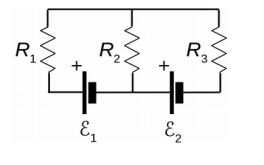
\includegraphics[scale=1.1]{ES5/SET052017.jpg}
	\end{center}
	\noindent\fbox{
		\parbox{\textwidth}{
			\null\hfill \textbf{Soluzione:} $R_x = 1\Omega$\\
			\textbf{Procedimento: } \\
			In questa tipologia di esercizio si deve impostare il sistema per poi trovare le rispettive correnti, per farlo bisogno stabilire arbitrariamente il verso della corrente di ogni maglia.\\
			 Nel nostro caso supporremo che la corrente viaggi in senso orario in entrambe le maglie.\\

			\systeme*{
				I_1=I_2 +I_3,
				\varepsilon_1= R_1\cdot I_1 + R_2\cdot I_2,
				\varepsilon_2= -R_2\cdot I_2 + R_3\cdot I_3
			}
			\\ \\
			Risolvendo il sistema si otterranno i valori delle correnti.\\ \\
			\systeme*{
				I_1=I_2 +I_3,
				1.5= 4\cdot I_1 + 6\cdot I_2,
				3= -6\cdot I_2 + 3\cdot I_3
			}
			\hspace{1.45cm} = \hspace{1.5cm}
			\systeme*{
				I_1=I_2 +I_3,
				1.5= 4\cdot I_2 + 4\cdot I_3 + 6\cdot I_2,
				3= -6\cdot I_2 + 3\cdot I_3
			}\\ \\
			\systeme*{
				I_1=I_2 +I_3,
				1.5= 10\cdot I_2 + 4\cdot I_3,
				I_3=\frac{3V +6\cdot I_2}{3}
			}
			\hspace{1.5cm} = \hspace{1.5cm}
			\systeme*{
				I_1=I_2 +I_3,
				1.5= 10\cdot I_2 + 4\cdot (1 +2\cdot I_2),
				3= -6\cdot I_2 + 3\cdot I_3
			}\\ \\
			\systeme*{
				I_1=I_2 +I_3,
				I_2= -0.139,
				I_3= 1 +2\cdot I_2
			}
			\hspace{2.45cm} = \hspace{1.45cm}
			\systeme*{
				I_1=-0.139 +I_3,
				I_2= -0.139,
				I_3= 0.722
			}\\ \\
			\systeme*{
				I_1= 0.583A,
				I_2= -0.139A,
				I_3= 0.722A
			}\\ \\
		}
	}	
	
\end{figure}
\begin{figure}[h!]
\textbf{Tema d'Esame di Gennaio 2018}\\ \\
Una persona di massa $70.0 kg$ sta su una bilancia posta all’equatore sulla
superficie di un pianeta (supposto perfettamente sferico e uniforme). Qual è il
peso misurato dalla bilancia se il diametro del pianeta è il doppio di quello della
terra, ma la sua densità media ed il suo periodo di rotazione sono gli stessi della
terra? ($M_T = 5.97\cdot 10^{24}kg, R_T = 6370 km, T_T = 24.0 h$) 
\end{figure}

\clearpage
\section{Tipologia Esercizio 3}
In particolare verranno trattati gli esercizi riguardanti:
\begin{itemize}
\item Gravitazione
\end{itemize}
\begin{figure}[h!]
\textbf{Tema d'Esame di Gennaio 2015}\\ \\
Si determini la differenza di potenziali ai capi della resistenza $R4$ del circuito mostrato in figura. La differenza di potenziale fornita dalla batteria è di $12V$ e i valori delle resistenze sono rispettivamente $R2=15\Omega, R3=40\Omega, R4=25\Omega, R5=R6=32\Omega, R1=R7=18\Omega$
\begin{center}
		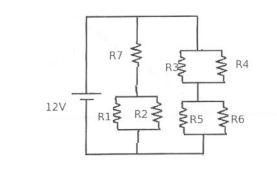
\includegraphics[scale=1.2]{ES5/GEN052015.jpg}
	\end{center}
	\begin{boxed}
		\null\hfill \textbf{Soluzione:} $V_4 = 5.85 V$\\
		\textbf{Procedimento: } \\
		Semplificazione delle Resistenze:\\
		$R_{34}=\frac{R_3\cdot R_4}{R_3+R_4}=\frac{40\Omega \cdot 25\Omega}{40\Omega+25\Omega}=15.38\Omega$\\
		$R_{56}=\frac{R_5\cdot R_6}{R_5+R_6}=\frac{32\Omega \cdot 32\Omega}{32\Omega+32\Omega}=16\Omega$\\
		$R_{12}=\frac{R_1\cdot R_2}{R_1+R_2}=\frac{18\Omega \cdot 15\Omega}{18\Omega+15\Omega}=8.18\Omega$\\
		$R_{127}=R_{12}+R_7=8.18\Omega + 18\Omega=26.18\Omega$\\
		$R_{3456}=R_{34}+R_{56}=15.38\Omega+16\Omega=31.38\Omega$\\
		$R_{tot}=\frac{R_{127}\cdot R_{3456}}{R_{127}+R_{3456}}=\frac{26.18\Omega \cdot 31.38\Omega}{26.18\Omega + 31.38\Omega}=14.23\Omega$\\
		Ricordando che la Tensione in parallelo non cambia, così come non cambia la corrente in serie:\\
		$V_{tot}=V_{127}=V_{3456}=12V$\\
		$I_{3456}=\frac{V_{3456}}{R_{3456}}=0.38A \qquad I_{3456}=I_{34}=I_{56}$\\
		$V_{34}=V_3=V_4=R_{34}\cdot I_{34}=15.38\Omega \cdot 0.38A=5.85\Omega \qquad V_{34}=V_3=V_4$
	\end{boxed}
\end{figure}

\begin{figure}[h!]
\textbf{Tema d'Esame di Febbraio 2015}\\ \\
 Nel circuito in figura, la corrente attraverso $R6$ è $i_6=1.40A$ e le resistenze sono
$R1=R2=R3=2.0\Omega, R4= 16.0\Omega, R5= 8.0 \Omega e R6= 4.0 \Omega$. Qual'è la forza elettromotrice della batteria (ideale)?
\begin{center}
		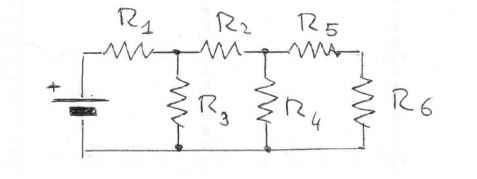
\includegraphics[scale=0.8]{ES5/FEB052015.jpg}
	\end{center}
\end{figure}

\begin{figure}[h!]
\textbf{Tema d'Esame di Giugno 2015}\\ \\
Si determini la differenza di potenziali ai capi della resistenza R4 del circuito mostrato in figura. La differenza di potenziale fornita dalla batteria è di $12V$ e i valori delle resistenze sono rispettivamente $R2=15\Omega, R3=40\Omega, R4=25\Omega, R5=R6=32\Omega, R1=R7=18\Omega$.
\begin{center}
		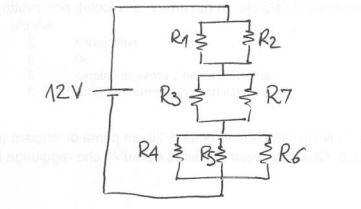
\includegraphics[scale=1]{ES5/GIU052015.jpg}
	\end{center}
\end{figure}

\begin{figure}[h!]
\textbf{Tema d'Esame di Luglio 2015}\\ \\
La differenza di potenziale fornita dalla batteria è di $12V$ e i valori delle resistenze sono rispettivamente $R2=15\Omega, R3=40\Omega, R4=25\Omega, R5=R6=32\Omega, R1=R7=18\Omega$
\begin{center}
		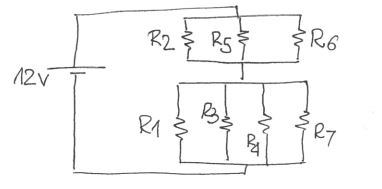
\includegraphics[scale=1]{ES5/LUG052015.jpg}
	\end{center}
\end{figure}

\begin{figure}[h!]
    \textbf{Tema d'Esame di Gennaio 2016}\\ \\
    Una molla viene compressa di 17 cm prima di lanciare una palla verso un piano inclinato
    senza attrito. La palla ha massa 1kg e il piano inclinato ha un'altezza H=1.28 m. Quanto vale
    la costante elastica della molla affinché la palla arrivi con una velocità di 4 m/s in cima al
    piano ?
    \\
        \begin{center}
            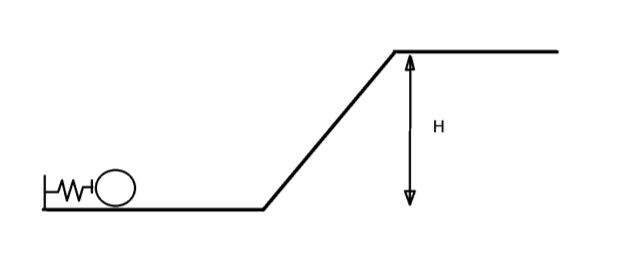
\includegraphics[scale=0.5]{ES2/GEN022016.jpg}
        \end{center}
    \end{figure}
    
    \begin{figure}[h!]
    \textbf{Tema d'Esame di Febbraio 2016}\\ \\
    Una palla di massa $250g$ è lanciata da una molla con costante elastica $63 N/m$ compressa di $45 cm$. La palla viaggia attraverso un piano inclinato alto $72 cm$. Una volta arrivata in cima al piano inclinato la palla incontra una superficie piatta frenante. Il coefficente d'attrito dinamico palla-superficie è di $m=0.42$. Che distanza percorre la palla sulla superficie frenante prima di fermarsi?
    \\
        \begin{center}
            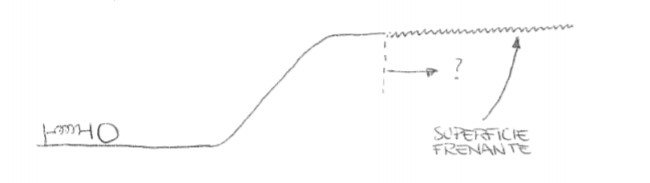
\includegraphics[scale=0.5]{ES2/FEB022016.jpg}
        \end{center}
        \noindent\fbox{
            \parbox{\textwidth}{
                \null\hfill \textbf{Soluzione:} $ s=4.477m $\\
                \textbf{Procedimento: } \\
                Trasformare le unità di misura:\\
                $\Delta x= 45cm =0.45m$\\
                $h=72cm=0.72m$\\ \\
                Impostando il seguente sistema, considerando come punto A la molla , il punto B il punto immediatamente dopo il piano inclinato e il punto C dove la palla si fermerà sul piano scabro.\\
                $$
                \begin{cases}
                    U_{El,A} = U_B + K_B \\
                    U_B + K_B = U_C + L_a
                \end{cases}
                =
                \begin{cases}
                    \frac{1}{2}\cdot k \cdot \Delta x^2 = m\cdot g \cdot h + \frac{1}{2} \cdot m \cdot v^2\\
                    \frac{1}{2}\cdot m \cdot v^2 = \mu_d \cdot m \cdot g \cdot cos(\alpha) \cdot \Delta s
                \end{cases}
                $$
                $$
                \begin{cases}
                    6.378J = 1.766J + 0.125kg \cdot v^2\\
                    0.125kg\cdot v^2 = 103N \cdot \Delta s
                \end{cases}
                =
                \begin{cases}
                    v^2 = 36.896 m^2/s^2 \\
                    \Delta s= 4.477m
                \end{cases}
                $$
                
            }
        }                  
    \end{figure}
    
    \begin{figure}[h!]
    \textbf{Tema d'Esame di Giugno 2016}\\ \\
    Una molla ideale può essere compressa di $1.0 m$ da una forza di $100 N$. La stessa molla è posta alla fine di un piano inclinato con attrito (coefficiente $0.2$) che forma un angolo di 30$^{\circ}$ con l'orizzontale. Una massa $M$ di $10 kg$ viene lasciata cadere da ferma dal vertice del piano inclinato e si arresta momentaneamente dopo aver compresso la molla di $2.0 m$. Qual'è la velocità della massa un attimo prima di toccare la molla? 
    \\
        \begin{center}
            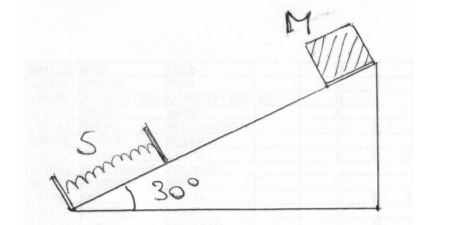
\includegraphics[scale=0.5]{ES2/GIU022016.jpg}
        \end{center}

        \noindent\fbox{
            \parbox{\textwidth}{
                \null\hfill \textbf{Soluzione:} $ s=6.324m/s $\\
                \textbf{Procedimento: } \\
                Trasformare le unità di misura:\\
                $\Delta x= 45cm =0.45m$\\
                $h=72cm=0.72m$\\ \\
                Impostando il seguente sistema, considerando come punto A la molla , il punto B dove parte il corpo.\\
                È conveniente ribaltare la struttura del problema per dire che la massa parte dalla molla e arriva nel punto B con velocità 0.\\
                $$
                \begin{cases}
                    U_{El,A} - L_a= U_B  \\
                    K_A - L_a = U_B
                \end{cases}
                =
                \begin{cases}
                    \frac{1}{2}\cdot k \cdot \Delta x^2 - \mu_d \cdot m \cdot g \cdot cos(\alpha) \cdot \Delta s= m\cdot g \cdot h \\
                    \frac{1}{2}\cdot m \cdot v^2 - \mu_d \cdot m \cdot g \cdot cos(\alpha) \cdot \Delta s=m\cdot g \cdot h
                \end{cases}
                $$
                Nota: con la seconda equazione del sistema ipotizziamo che a prescindere che sia stata spinta da una molla, calcoliamo la velocità necessaria che serve per spingere un corpo su una superficie scabra. \\
                A questo punto basta solamente eguagliare:\\
                $\frac{1}{2}\cdot k \cdot \Delta x^2 = \frac{1}{2}\cdot m \cdot v^2 \quad 200J=5kg\cdot v^2 \quad v=\sqrt{40m^2 /s^2}=6.324m/s$\\

               
                
            }
        }    
    \end{figure}
    
    \begin{figure}[h!]
    \textbf{Tema d'Esame di Luglio 2016}\\ \\
    La molla della figura ha una costante elastica $k = 120 \frac{N}{m}$ e una lunghezza a riposo di $45cm$. Quando un blocco di massa $M$ viene attaccato alla molla l'estensione di equilibrio della molla è $60cm$. Il piano inclinato è liscio(senza attrito) e forma un angolo di $40^\circ$ con l'orizzontale. Se la massa viene tirata leggermente verso il basso e viene rilasciata, qual è il periodo di oscillazione? 
    \\
        \begin{center}
            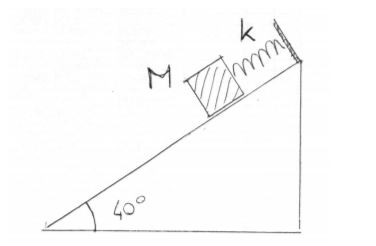
\includegraphics[scale=0.5]{ES2/LUG022016.jpg}
        \end{center}
    \end{figure}
    
    
\begin{figure}[h!]
\textbf{Tema d'Esame di Febbraio 2017}\\ \\
Sapendo che la resistenza $R8$ è attraversata da una corrente $i_8 = 0.20 A$, si calcoli la corrente che attraversa $R3$. Si considerino le seguenti resistenze $R8 = 10 \Omega, R1 = R2 = R3 = 5.0 \Omega , R4 = 12 \Omega , R5 = 15 \Omega $.
	\begin{center}
		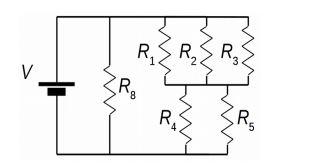
\includegraphics[scale=1.1]{ES5/FEB052017.jpg}
	\end{center}
	\noindent\fbox{
		\parbox{\textwidth}{
			\null\hfill \textbf{Soluzione:} $I_3 = 0.08A$\\
			\textbf{Procedimento: } \\
			Semplificazione delle Resistenze:\\
			$R_{123}=\frac{1}{\frac{1}{R_1}+\frac{1}{R_2}+\frac{1}{R_3}}=\frac{1}{\frac{1}{5\Omega}+\frac{1}{5\Omega}+\frac{1}{5\Omega}}=1.67\Omega$\\ \\ 
			$R_{45}=\frac{R_4\cdot R_5}{R_4 + R_5}=\frac{12\Omega\cdot 15\Omega}{12\Omega + 15\Omega}=6.67\Omega$\\
			$R_{12345}=R_{123}+R_{45}=6.67\Omega+1.67\Omega=8.34\Omega$\\
			Ricordando che la tensione in parallelo non cambia, così come non cambia la corrente in serie:\\
			$V_{tot}=V_{12345}=V_8=R_8\cdot I_8=10\Omega\cdot 0.2A=2V$\\
			$I_{12345}=I_{123}=I_{45}=\frac{V}{R_{12345}}=\frac{2V}{8.34\Omega}=0.24A$\\
			$V_{123}=R_{123}\cdot I_{12345}=1.67\Omega\cdot 0.24A=0.40V$\\
			$I_3=\frac{V_{123}}{R_3}=\frac{0.40V}{5\Omega}=0.08A$
		}
	}	
	
\end{figure}

\begin{figure}[h!]
\textbf{Tema d'Esame di Giugno 2017}\\ \\
 Si determini il valore della resistenza $R_x$ del circuito mostrato nella figura sotto a sinistra. La differenza di potenziale fornita dalla batteria è $3 V$, la corrente $i_3$ che scorre nella resistenza $R_3$ è pari a $0.1 A$ ed i valori delle altre resistenze nel circuito
sono $R1 = R2 = 5 \Omega ,R3 = R4 = 10 \Omega$.
	\begin{center}
		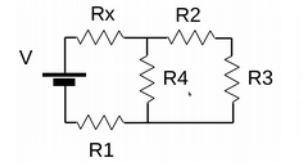
\includegraphics[scale=1.1]{ES5/GIU052017.jpg}
	\end{center}
	\noindent\fbox{
		\parbox{\textwidth}{
			\null\hfill \textbf{Soluzione:} $R_x = 1\Omega$\\
			\textbf{Procedimento: } \\
			Ricordando che la tensione in parallelo non cambia, così come non cambia la corrente in serie proseguiamo semplificando le resistenze e aggiornando man mano corrente e tensione:\\
			
			
			$R_{23}=R_2 + R_3=5\Omega + 10\Omega=15\Omega$\\
			$I_3=I_2=I_{23}=0.1A$\\
			$V_{23}=V_{234}=V_4=R_{23} \cdot I_{23}=15\Omega \cdot 0.1A=1.5V$\\
			$I_{234}=\frac{V_{234}}{R_{234}}=\frac{1.5V}{6\Omega}=0.25A$\\
			$V_1=R_1\cdot I_{234}=5\Omega \cdot 0.25A=1.25V$\\
			$V_x=V_{tot}- V_1 - V_{234}=3V - 1.25V -1.5V=0.25V$\\
			$R_x=\frac{V_x}{I_{234}}=\frac{0.25V}{0.25A}=1\Omega$
		}
	}	
\end{figure}

\begin{figure}[h!]
\textbf{Tema d'Esame di Settembre 2017}\\ \\
Trovare le correnti $i_1, i_2 , i_3$ nei tre rami del circuito qui sotto.
$R1 = 4.0 \Omega, R2 = 6.0 \Omega, R3 = 3.0 \Omega$ ed $ E 1 = 1.5 V,  E 2 = 3.0 V$.
	\begin{center}
		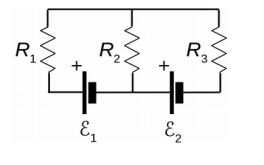
\includegraphics[scale=1.1]{ES5/SET052017.jpg}
	\end{center}
	\noindent\fbox{
		\parbox{\textwidth}{
			\null\hfill \textbf{Soluzione:} $R_x = 1\Omega$\\
			\textbf{Procedimento: } \\
			In questa tipologia di esercizio si deve impostare il sistema per poi trovare le rispettive correnti, per farlo bisogno stabilire arbitrariamente il verso della corrente di ogni maglia.\\
			 Nel nostro caso supporremo che la corrente viaggi in senso orario in entrambe le maglie.\\

			\systeme*{
				I_1=I_2 +I_3,
				\varepsilon_1= R_1\cdot I_1 + R_2\cdot I_2,
				\varepsilon_2= -R_2\cdot I_2 + R_3\cdot I_3
			}
			\\ \\
			Risolvendo il sistema si otterranno i valori delle correnti.\\ \\
			\systeme*{
				I_1=I_2 +I_3,
				1.5= 4\cdot I_1 + 6\cdot I_2,
				3= -6\cdot I_2 + 3\cdot I_3
			}
			\hspace{1.45cm} = \hspace{1.5cm}
			\systeme*{
				I_1=I_2 +I_3,
				1.5= 4\cdot I_2 + 4\cdot I_3 + 6\cdot I_2,
				3= -6\cdot I_2 + 3\cdot I_3
			}\\ \\
			\systeme*{
				I_1=I_2 +I_3,
				1.5= 10\cdot I_2 + 4\cdot I_3,
				I_3=\frac{3V +6\cdot I_2}{3}
			}
			\hspace{1.5cm} = \hspace{1.5cm}
			\systeme*{
				I_1=I_2 +I_3,
				1.5= 10\cdot I_2 + 4\cdot (1 +2\cdot I_2),
				3= -6\cdot I_2 + 3\cdot I_3
			}\\ \\
			\systeme*{
				I_1=I_2 +I_3,
				I_2= -0.139,
				I_3= 1 +2\cdot I_2
			}
			\hspace{2.45cm} = \hspace{1.45cm}
			\systeme*{
				I_1=-0.139 +I_3,
				I_2= -0.139,
				I_3= 0.722
			}\\ \\
			\systeme*{
				I_1= 0.583A,
				I_2= -0.139A,
				I_3= 0.722A
			}\\ \\
		}
	}	
	
\end{figure}
\begin{figure}[h!]
\textbf{Tema d'Esame di Gennaio 2018}\\ \\
Una persona di massa $70.0 kg$ sta su una bilancia posta all’equatore sulla
superficie di un pianeta (supposto perfettamente sferico e uniforme). Qual è il
peso misurato dalla bilancia se il diametro del pianeta è il doppio di quello della
terra, ma la sua densità media ed il suo periodo di rotazione sono gli stessi della
terra? ($M_T = 5.97\cdot 10^{24}kg, R_T = 6370 km, T_T = 24.0 h$) 
\end{figure}
\clearpage

\section{Tipologia Esercizio 4}
In particolare verranno trattati gli esercizi riguardanti:
\begin{itemize}
\item Fluidi
\end{itemize}
\begin{figure}[h!]
\textbf{Tema d'Esame di Gennaio 2015}\\ \\
Si determini la differenza di potenziali ai capi della resistenza $R4$ del circuito mostrato in figura. La differenza di potenziale fornita dalla batteria è di $12V$ e i valori delle resistenze sono rispettivamente $R2=15\Omega, R3=40\Omega, R4=25\Omega, R5=R6=32\Omega, R1=R7=18\Omega$
\begin{center}
		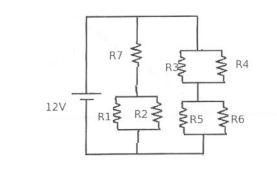
\includegraphics[scale=1.2]{ES5/GEN052015.jpg}
	\end{center}
	\begin{boxed}
		\null\hfill \textbf{Soluzione:} $V_4 = 5.85 V$\\
		\textbf{Procedimento: } \\
		Semplificazione delle Resistenze:\\
		$R_{34}=\frac{R_3\cdot R_4}{R_3+R_4}=\frac{40\Omega \cdot 25\Omega}{40\Omega+25\Omega}=15.38\Omega$\\
		$R_{56}=\frac{R_5\cdot R_6}{R_5+R_6}=\frac{32\Omega \cdot 32\Omega}{32\Omega+32\Omega}=16\Omega$\\
		$R_{12}=\frac{R_1\cdot R_2}{R_1+R_2}=\frac{18\Omega \cdot 15\Omega}{18\Omega+15\Omega}=8.18\Omega$\\
		$R_{127}=R_{12}+R_7=8.18\Omega + 18\Omega=26.18\Omega$\\
		$R_{3456}=R_{34}+R_{56}=15.38\Omega+16\Omega=31.38\Omega$\\
		$R_{tot}=\frac{R_{127}\cdot R_{3456}}{R_{127}+R_{3456}}=\frac{26.18\Omega \cdot 31.38\Omega}{26.18\Omega + 31.38\Omega}=14.23\Omega$\\
		Ricordando che la Tensione in parallelo non cambia, così come non cambia la corrente in serie:\\
		$V_{tot}=V_{127}=V_{3456}=12V$\\
		$I_{3456}=\frac{V_{3456}}{R_{3456}}=0.38A \qquad I_{3456}=I_{34}=I_{56}$\\
		$V_{34}=V_3=V_4=R_{34}\cdot I_{34}=15.38\Omega \cdot 0.38A=5.85\Omega \qquad V_{34}=V_3=V_4$
	\end{boxed}
\end{figure}

\begin{figure}[h!]
\textbf{Tema d'Esame di Febbraio 2015}\\ \\
 Nel circuito in figura, la corrente attraverso $R6$ è $i_6=1.40A$ e le resistenze sono
$R1=R2=R3=2.0\Omega, R4= 16.0\Omega, R5= 8.0 \Omega e R6= 4.0 \Omega$. Qual'è la forza elettromotrice della batteria (ideale)?
\begin{center}
		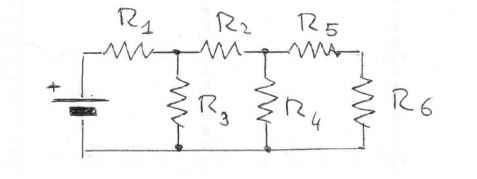
\includegraphics[scale=0.8]{ES5/FEB052015.jpg}
	\end{center}
\end{figure}

\begin{figure}[h!]
\textbf{Tema d'Esame di Giugno 2015}\\ \\
Si determini la differenza di potenziali ai capi della resistenza R4 del circuito mostrato in figura. La differenza di potenziale fornita dalla batteria è di $12V$ e i valori delle resistenze sono rispettivamente $R2=15\Omega, R3=40\Omega, R4=25\Omega, R5=R6=32\Omega, R1=R7=18\Omega$.
\begin{center}
		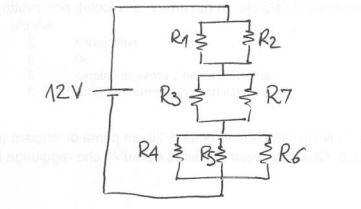
\includegraphics[scale=1]{ES5/GIU052015.jpg}
	\end{center}
\end{figure}

\begin{figure}[h!]
\textbf{Tema d'Esame di Luglio 2015}\\ \\
La differenza di potenziale fornita dalla batteria è di $12V$ e i valori delle resistenze sono rispettivamente $R2=15\Omega, R3=40\Omega, R4=25\Omega, R5=R6=32\Omega, R1=R7=18\Omega$
\begin{center}
		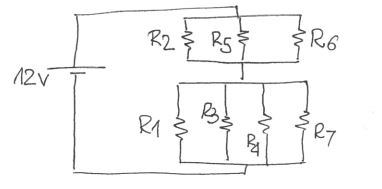
\includegraphics[scale=1]{ES5/LUG052015.jpg}
	\end{center}
\end{figure}

\begin{figure}[h!]
    \textbf{Tema d'Esame di Gennaio 2016}\\ \\
    Una molla viene compressa di 17 cm prima di lanciare una palla verso un piano inclinato
    senza attrito. La palla ha massa 1kg e il piano inclinato ha un'altezza H=1.28 m. Quanto vale
    la costante elastica della molla affinché la palla arrivi con una velocità di 4 m/s in cima al
    piano ?
    \\
        \begin{center}
            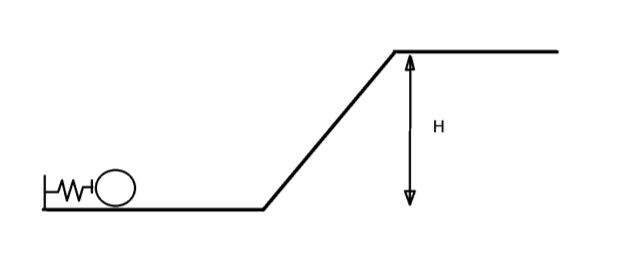
\includegraphics[scale=0.5]{ES2/GEN022016.jpg}
        \end{center}
    \end{figure}
    
    \begin{figure}[h!]
    \textbf{Tema d'Esame di Febbraio 2016}\\ \\
    Una palla di massa $250g$ è lanciata da una molla con costante elastica $63 N/m$ compressa di $45 cm$. La palla viaggia attraverso un piano inclinato alto $72 cm$. Una volta arrivata in cima al piano inclinato la palla incontra una superficie piatta frenante. Il coefficente d'attrito dinamico palla-superficie è di $m=0.42$. Che distanza percorre la palla sulla superficie frenante prima di fermarsi?
    \\
        \begin{center}
            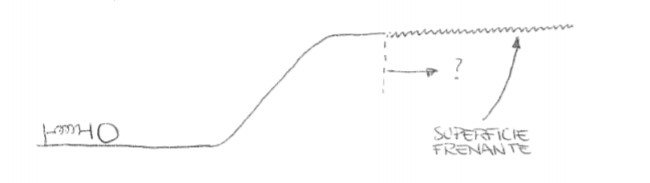
\includegraphics[scale=0.5]{ES2/FEB022016.jpg}
        \end{center}
        \noindent\fbox{
            \parbox{\textwidth}{
                \null\hfill \textbf{Soluzione:} $ s=4.477m $\\
                \textbf{Procedimento: } \\
                Trasformare le unità di misura:\\
                $\Delta x= 45cm =0.45m$\\
                $h=72cm=0.72m$\\ \\
                Impostando il seguente sistema, considerando come punto A la molla , il punto B il punto immediatamente dopo il piano inclinato e il punto C dove la palla si fermerà sul piano scabro.\\
                $$
                \begin{cases}
                    U_{El,A} = U_B + K_B \\
                    U_B + K_B = U_C + L_a
                \end{cases}
                =
                \begin{cases}
                    \frac{1}{2}\cdot k \cdot \Delta x^2 = m\cdot g \cdot h + \frac{1}{2} \cdot m \cdot v^2\\
                    \frac{1}{2}\cdot m \cdot v^2 = \mu_d \cdot m \cdot g \cdot cos(\alpha) \cdot \Delta s
                \end{cases}
                $$
                $$
                \begin{cases}
                    6.378J = 1.766J + 0.125kg \cdot v^2\\
                    0.125kg\cdot v^2 = 103N \cdot \Delta s
                \end{cases}
                =
                \begin{cases}
                    v^2 = 36.896 m^2/s^2 \\
                    \Delta s= 4.477m
                \end{cases}
                $$
                
            }
        }                  
    \end{figure}
    
    \begin{figure}[h!]
    \textbf{Tema d'Esame di Giugno 2016}\\ \\
    Una molla ideale può essere compressa di $1.0 m$ da una forza di $100 N$. La stessa molla è posta alla fine di un piano inclinato con attrito (coefficiente $0.2$) che forma un angolo di 30$^{\circ}$ con l'orizzontale. Una massa $M$ di $10 kg$ viene lasciata cadere da ferma dal vertice del piano inclinato e si arresta momentaneamente dopo aver compresso la molla di $2.0 m$. Qual'è la velocità della massa un attimo prima di toccare la molla? 
    \\
        \begin{center}
            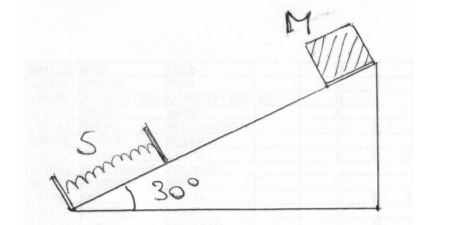
\includegraphics[scale=0.5]{ES2/GIU022016.jpg}
        \end{center}

        \noindent\fbox{
            \parbox{\textwidth}{
                \null\hfill \textbf{Soluzione:} $ s=6.324m/s $\\
                \textbf{Procedimento: } \\
                Trasformare le unità di misura:\\
                $\Delta x= 45cm =0.45m$\\
                $h=72cm=0.72m$\\ \\
                Impostando il seguente sistema, considerando come punto A la molla , il punto B dove parte il corpo.\\
                È conveniente ribaltare la struttura del problema per dire che la massa parte dalla molla e arriva nel punto B con velocità 0.\\
                $$
                \begin{cases}
                    U_{El,A} - L_a= U_B  \\
                    K_A - L_a = U_B
                \end{cases}
                =
                \begin{cases}
                    \frac{1}{2}\cdot k \cdot \Delta x^2 - \mu_d \cdot m \cdot g \cdot cos(\alpha) \cdot \Delta s= m\cdot g \cdot h \\
                    \frac{1}{2}\cdot m \cdot v^2 - \mu_d \cdot m \cdot g \cdot cos(\alpha) \cdot \Delta s=m\cdot g \cdot h
                \end{cases}
                $$
                Nota: con la seconda equazione del sistema ipotizziamo che a prescindere che sia stata spinta da una molla, calcoliamo la velocità necessaria che serve per spingere un corpo su una superficie scabra. \\
                A questo punto basta solamente eguagliare:\\
                $\frac{1}{2}\cdot k \cdot \Delta x^2 = \frac{1}{2}\cdot m \cdot v^2 \quad 200J=5kg\cdot v^2 \quad v=\sqrt{40m^2 /s^2}=6.324m/s$\\

               
                
            }
        }    
    \end{figure}
    
    \begin{figure}[h!]
    \textbf{Tema d'Esame di Luglio 2016}\\ \\
    La molla della figura ha una costante elastica $k = 120 \frac{N}{m}$ e una lunghezza a riposo di $45cm$. Quando un blocco di massa $M$ viene attaccato alla molla l'estensione di equilibrio della molla è $60cm$. Il piano inclinato è liscio(senza attrito) e forma un angolo di $40^\circ$ con l'orizzontale. Se la massa viene tirata leggermente verso il basso e viene rilasciata, qual è il periodo di oscillazione? 
    \\
        \begin{center}
            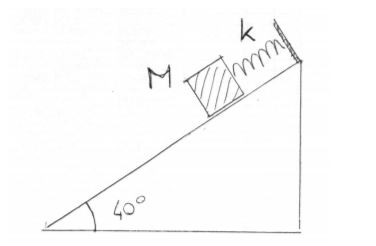
\includegraphics[scale=0.5]{ES2/LUG022016.jpg}
        \end{center}
    \end{figure}
    
    
\begin{figure}[h!]
\textbf{Tema d'Esame di Febbraio 2017}\\ \\
Sapendo che la resistenza $R8$ è attraversata da una corrente $i_8 = 0.20 A$, si calcoli la corrente che attraversa $R3$. Si considerino le seguenti resistenze $R8 = 10 \Omega, R1 = R2 = R3 = 5.0 \Omega , R4 = 12 \Omega , R5 = 15 \Omega $.
	\begin{center}
		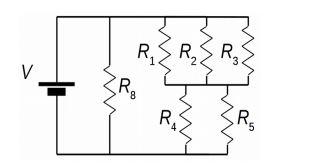
\includegraphics[scale=1.1]{ES5/FEB052017.jpg}
	\end{center}
	\noindent\fbox{
		\parbox{\textwidth}{
			\null\hfill \textbf{Soluzione:} $I_3 = 0.08A$\\
			\textbf{Procedimento: } \\
			Semplificazione delle Resistenze:\\
			$R_{123}=\frac{1}{\frac{1}{R_1}+\frac{1}{R_2}+\frac{1}{R_3}}=\frac{1}{\frac{1}{5\Omega}+\frac{1}{5\Omega}+\frac{1}{5\Omega}}=1.67\Omega$\\ \\ 
			$R_{45}=\frac{R_4\cdot R_5}{R_4 + R_5}=\frac{12\Omega\cdot 15\Omega}{12\Omega + 15\Omega}=6.67\Omega$\\
			$R_{12345}=R_{123}+R_{45}=6.67\Omega+1.67\Omega=8.34\Omega$\\
			Ricordando che la tensione in parallelo non cambia, così come non cambia la corrente in serie:\\
			$V_{tot}=V_{12345}=V_8=R_8\cdot I_8=10\Omega\cdot 0.2A=2V$\\
			$I_{12345}=I_{123}=I_{45}=\frac{V}{R_{12345}}=\frac{2V}{8.34\Omega}=0.24A$\\
			$V_{123}=R_{123}\cdot I_{12345}=1.67\Omega\cdot 0.24A=0.40V$\\
			$I_3=\frac{V_{123}}{R_3}=\frac{0.40V}{5\Omega}=0.08A$
		}
	}	
	
\end{figure}

\begin{figure}[h!]
\textbf{Tema d'Esame di Giugno 2017}\\ \\
 Si determini il valore della resistenza $R_x$ del circuito mostrato nella figura sotto a sinistra. La differenza di potenziale fornita dalla batteria è $3 V$, la corrente $i_3$ che scorre nella resistenza $R_3$ è pari a $0.1 A$ ed i valori delle altre resistenze nel circuito
sono $R1 = R2 = 5 \Omega ,R3 = R4 = 10 \Omega$.
	\begin{center}
		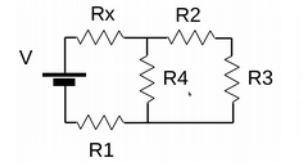
\includegraphics[scale=1.1]{ES5/GIU052017.jpg}
	\end{center}
	\noindent\fbox{
		\parbox{\textwidth}{
			\null\hfill \textbf{Soluzione:} $R_x = 1\Omega$\\
			\textbf{Procedimento: } \\
			Ricordando che la tensione in parallelo non cambia, così come non cambia la corrente in serie proseguiamo semplificando le resistenze e aggiornando man mano corrente e tensione:\\
			
			
			$R_{23}=R_2 + R_3=5\Omega + 10\Omega=15\Omega$\\
			$I_3=I_2=I_{23}=0.1A$\\
			$V_{23}=V_{234}=V_4=R_{23} \cdot I_{23}=15\Omega \cdot 0.1A=1.5V$\\
			$I_{234}=\frac{V_{234}}{R_{234}}=\frac{1.5V}{6\Omega}=0.25A$\\
			$V_1=R_1\cdot I_{234}=5\Omega \cdot 0.25A=1.25V$\\
			$V_x=V_{tot}- V_1 - V_{234}=3V - 1.25V -1.5V=0.25V$\\
			$R_x=\frac{V_x}{I_{234}}=\frac{0.25V}{0.25A}=1\Omega$
		}
	}	
\end{figure}

\begin{figure}[h!]
\textbf{Tema d'Esame di Settembre 2017}\\ \\
Trovare le correnti $i_1, i_2 , i_3$ nei tre rami del circuito qui sotto.
$R1 = 4.0 \Omega, R2 = 6.0 \Omega, R3 = 3.0 \Omega$ ed $ E 1 = 1.5 V,  E 2 = 3.0 V$.
	\begin{center}
		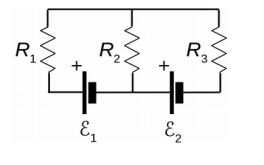
\includegraphics[scale=1.1]{ES5/SET052017.jpg}
	\end{center}
	\noindent\fbox{
		\parbox{\textwidth}{
			\null\hfill \textbf{Soluzione:} $R_x = 1\Omega$\\
			\textbf{Procedimento: } \\
			In questa tipologia di esercizio si deve impostare il sistema per poi trovare le rispettive correnti, per farlo bisogno stabilire arbitrariamente il verso della corrente di ogni maglia.\\
			 Nel nostro caso supporremo che la corrente viaggi in senso orario in entrambe le maglie.\\

			\systeme*{
				I_1=I_2 +I_3,
				\varepsilon_1= R_1\cdot I_1 + R_2\cdot I_2,
				\varepsilon_2= -R_2\cdot I_2 + R_3\cdot I_3
			}
			\\ \\
			Risolvendo il sistema si otterranno i valori delle correnti.\\ \\
			\systeme*{
				I_1=I_2 +I_3,
				1.5= 4\cdot I_1 + 6\cdot I_2,
				3= -6\cdot I_2 + 3\cdot I_3
			}
			\hspace{1.45cm} = \hspace{1.5cm}
			\systeme*{
				I_1=I_2 +I_3,
				1.5= 4\cdot I_2 + 4\cdot I_3 + 6\cdot I_2,
				3= -6\cdot I_2 + 3\cdot I_3
			}\\ \\
			\systeme*{
				I_1=I_2 +I_3,
				1.5= 10\cdot I_2 + 4\cdot I_3,
				I_3=\frac{3V +6\cdot I_2}{3}
			}
			\hspace{1.5cm} = \hspace{1.5cm}
			\systeme*{
				I_1=I_2 +I_3,
				1.5= 10\cdot I_2 + 4\cdot (1 +2\cdot I_2),
				3= -6\cdot I_2 + 3\cdot I_3
			}\\ \\
			\systeme*{
				I_1=I_2 +I_3,
				I_2= -0.139,
				I_3= 1 +2\cdot I_2
			}
			\hspace{2.45cm} = \hspace{1.45cm}
			\systeme*{
				I_1=-0.139 +I_3,
				I_2= -0.139,
				I_3= 0.722
			}\\ \\
			\systeme*{
				I_1= 0.583A,
				I_2= -0.139A,
				I_3= 0.722A
			}\\ \\
		}
	}	
	
\end{figure}
\begin{figure}[h!]
\textbf{Tema d'Esame di Gennaio 2018}\\ \\
Una persona di massa $70.0 kg$ sta su una bilancia posta all’equatore sulla
superficie di un pianeta (supposto perfettamente sferico e uniforme). Qual è il
peso misurato dalla bilancia se il diametro del pianeta è il doppio di quello della
terra, ma la sua densità media ed il suo periodo di rotazione sono gli stessi della
terra? ($M_T = 5.97\cdot 10^{24}kg, R_T = 6370 km, T_T = 24.0 h$) 
\end{figure}
\clearpage
\section{Tipologia Esercizio 5}
In particolare verranno trattati gli esercizi riguardanti:
\begin{itemize}
\item Circuiti 
\end{itemize}
\begin{figure}[h!]
\textbf{Tema d'Esame di Gennaio 2015}\\ \\
Si determini la differenza di potenziali ai capi della resistenza $R4$ del circuito mostrato in figura. La differenza di potenziale fornita dalla batteria è di $12V$ e i valori delle resistenze sono rispettivamente $R2=15\Omega, R3=40\Omega, R4=25\Omega, R5=R6=32\Omega, R1=R7=18\Omega$
\begin{center}
		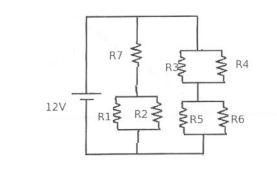
\includegraphics[scale=1.2]{ES5/GEN052015.jpg}
	\end{center}
	\begin{boxed}
		\null\hfill \textbf{Soluzione:} $V_4 = 5.85 V$\\
		\textbf{Procedimento: } \\
		Semplificazione delle Resistenze:\\
		$R_{34}=\frac{R_3\cdot R_4}{R_3+R_4}=\frac{40\Omega \cdot 25\Omega}{40\Omega+25\Omega}=15.38\Omega$\\
		$R_{56}=\frac{R_5\cdot R_6}{R_5+R_6}=\frac{32\Omega \cdot 32\Omega}{32\Omega+32\Omega}=16\Omega$\\
		$R_{12}=\frac{R_1\cdot R_2}{R_1+R_2}=\frac{18\Omega \cdot 15\Omega}{18\Omega+15\Omega}=8.18\Omega$\\
		$R_{127}=R_{12}+R_7=8.18\Omega + 18\Omega=26.18\Omega$\\
		$R_{3456}=R_{34}+R_{56}=15.38\Omega+16\Omega=31.38\Omega$\\
		$R_{tot}=\frac{R_{127}\cdot R_{3456}}{R_{127}+R_{3456}}=\frac{26.18\Omega \cdot 31.38\Omega}{26.18\Omega + 31.38\Omega}=14.23\Omega$\\
		Ricordando che la Tensione in parallelo non cambia, così come non cambia la corrente in serie:\\
		$V_{tot}=V_{127}=V_{3456}=12V$\\
		$I_{3456}=\frac{V_{3456}}{R_{3456}}=0.38A \qquad I_{3456}=I_{34}=I_{56}$\\
		$V_{34}=V_3=V_4=R_{34}\cdot I_{34}=15.38\Omega \cdot 0.38A=5.85\Omega \qquad V_{34}=V_3=V_4$
	\end{boxed}
\end{figure}

\begin{figure}[h!]
\textbf{Tema d'Esame di Febbraio 2015}\\ \\
 Nel circuito in figura, la corrente attraverso $R6$ è $i_6=1.40A$ e le resistenze sono
$R1=R2=R3=2.0\Omega, R4= 16.0\Omega, R5= 8.0 \Omega e R6= 4.0 \Omega$. Qual'è la forza elettromotrice della batteria (ideale)?
\begin{center}
		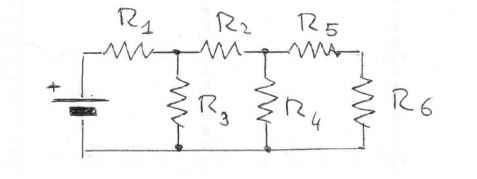
\includegraphics[scale=0.8]{ES5/FEB052015.jpg}
	\end{center}
\end{figure}

\begin{figure}[h!]
\textbf{Tema d'Esame di Giugno 2015}\\ \\
Si determini la differenza di potenziali ai capi della resistenza R4 del circuito mostrato in figura. La differenza di potenziale fornita dalla batteria è di $12V$ e i valori delle resistenze sono rispettivamente $R2=15\Omega, R3=40\Omega, R4=25\Omega, R5=R6=32\Omega, R1=R7=18\Omega$.
\begin{center}
		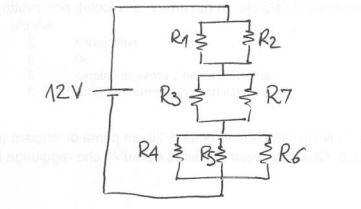
\includegraphics[scale=1]{ES5/GIU052015.jpg}
	\end{center}
\end{figure}

\begin{figure}[h!]
\textbf{Tema d'Esame di Luglio 2015}\\ \\
La differenza di potenziale fornita dalla batteria è di $12V$ e i valori delle resistenze sono rispettivamente $R2=15\Omega, R3=40\Omega, R4=25\Omega, R5=R6=32\Omega, R1=R7=18\Omega$
\begin{center}
		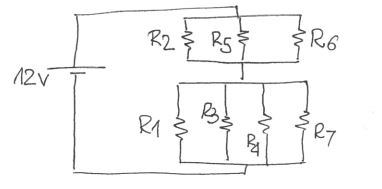
\includegraphics[scale=1]{ES5/LUG052015.jpg}
	\end{center}
\end{figure}

\begin{figure}[h!]
    \textbf{Tema d'Esame di Gennaio 2016}\\ \\
    Una molla viene compressa di 17 cm prima di lanciare una palla verso un piano inclinato
    senza attrito. La palla ha massa 1kg e il piano inclinato ha un'altezza H=1.28 m. Quanto vale
    la costante elastica della molla affinché la palla arrivi con una velocità di 4 m/s in cima al
    piano ?
    \\
        \begin{center}
            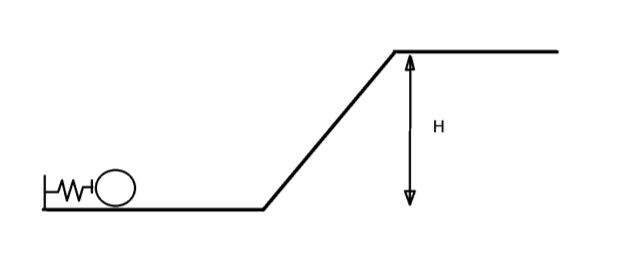
\includegraphics[scale=0.5]{ES2/GEN022016.jpg}
        \end{center}
    \end{figure}
    
    \begin{figure}[h!]
    \textbf{Tema d'Esame di Febbraio 2016}\\ \\
    Una palla di massa $250g$ è lanciata da una molla con costante elastica $63 N/m$ compressa di $45 cm$. La palla viaggia attraverso un piano inclinato alto $72 cm$. Una volta arrivata in cima al piano inclinato la palla incontra una superficie piatta frenante. Il coefficente d'attrito dinamico palla-superficie è di $m=0.42$. Che distanza percorre la palla sulla superficie frenante prima di fermarsi?
    \\
        \begin{center}
            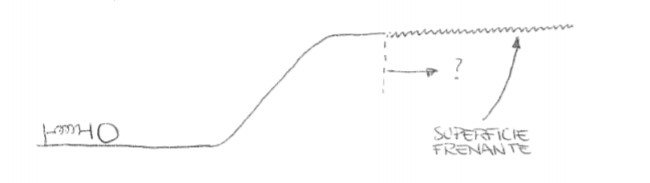
\includegraphics[scale=0.5]{ES2/FEB022016.jpg}
        \end{center}
        \noindent\fbox{
            \parbox{\textwidth}{
                \null\hfill \textbf{Soluzione:} $ s=4.477m $\\
                \textbf{Procedimento: } \\
                Trasformare le unità di misura:\\
                $\Delta x= 45cm =0.45m$\\
                $h=72cm=0.72m$\\ \\
                Impostando il seguente sistema, considerando come punto A la molla , il punto B il punto immediatamente dopo il piano inclinato e il punto C dove la palla si fermerà sul piano scabro.\\
                $$
                \begin{cases}
                    U_{El,A} = U_B + K_B \\
                    U_B + K_B = U_C + L_a
                \end{cases}
                =
                \begin{cases}
                    \frac{1}{2}\cdot k \cdot \Delta x^2 = m\cdot g \cdot h + \frac{1}{2} \cdot m \cdot v^2\\
                    \frac{1}{2}\cdot m \cdot v^2 = \mu_d \cdot m \cdot g \cdot cos(\alpha) \cdot \Delta s
                \end{cases}
                $$
                $$
                \begin{cases}
                    6.378J = 1.766J + 0.125kg \cdot v^2\\
                    0.125kg\cdot v^2 = 103N \cdot \Delta s
                \end{cases}
                =
                \begin{cases}
                    v^2 = 36.896 m^2/s^2 \\
                    \Delta s= 4.477m
                \end{cases}
                $$
                
            }
        }                  
    \end{figure}
    
    \begin{figure}[h!]
    \textbf{Tema d'Esame di Giugno 2016}\\ \\
    Una molla ideale può essere compressa di $1.0 m$ da una forza di $100 N$. La stessa molla è posta alla fine di un piano inclinato con attrito (coefficiente $0.2$) che forma un angolo di 30$^{\circ}$ con l'orizzontale. Una massa $M$ di $10 kg$ viene lasciata cadere da ferma dal vertice del piano inclinato e si arresta momentaneamente dopo aver compresso la molla di $2.0 m$. Qual'è la velocità della massa un attimo prima di toccare la molla? 
    \\
        \begin{center}
            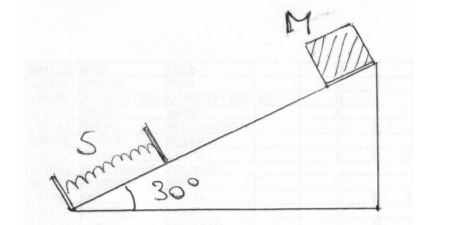
\includegraphics[scale=0.5]{ES2/GIU022016.jpg}
        \end{center}

        \noindent\fbox{
            \parbox{\textwidth}{
                \null\hfill \textbf{Soluzione:} $ s=6.324m/s $\\
                \textbf{Procedimento: } \\
                Trasformare le unità di misura:\\
                $\Delta x= 45cm =0.45m$\\
                $h=72cm=0.72m$\\ \\
                Impostando il seguente sistema, considerando come punto A la molla , il punto B dove parte il corpo.\\
                È conveniente ribaltare la struttura del problema per dire che la massa parte dalla molla e arriva nel punto B con velocità 0.\\
                $$
                \begin{cases}
                    U_{El,A} - L_a= U_B  \\
                    K_A - L_a = U_B
                \end{cases}
                =
                \begin{cases}
                    \frac{1}{2}\cdot k \cdot \Delta x^2 - \mu_d \cdot m \cdot g \cdot cos(\alpha) \cdot \Delta s= m\cdot g \cdot h \\
                    \frac{1}{2}\cdot m \cdot v^2 - \mu_d \cdot m \cdot g \cdot cos(\alpha) \cdot \Delta s=m\cdot g \cdot h
                \end{cases}
                $$
                Nota: con la seconda equazione del sistema ipotizziamo che a prescindere che sia stata spinta da una molla, calcoliamo la velocità necessaria che serve per spingere un corpo su una superficie scabra. \\
                A questo punto basta solamente eguagliare:\\
                $\frac{1}{2}\cdot k \cdot \Delta x^2 = \frac{1}{2}\cdot m \cdot v^2 \quad 200J=5kg\cdot v^2 \quad v=\sqrt{40m^2 /s^2}=6.324m/s$\\

               
                
            }
        }    
    \end{figure}
    
    \begin{figure}[h!]
    \textbf{Tema d'Esame di Luglio 2016}\\ \\
    La molla della figura ha una costante elastica $k = 120 \frac{N}{m}$ e una lunghezza a riposo di $45cm$. Quando un blocco di massa $M$ viene attaccato alla molla l'estensione di equilibrio della molla è $60cm$. Il piano inclinato è liscio(senza attrito) e forma un angolo di $40^\circ$ con l'orizzontale. Se la massa viene tirata leggermente verso il basso e viene rilasciata, qual è il periodo di oscillazione? 
    \\
        \begin{center}
            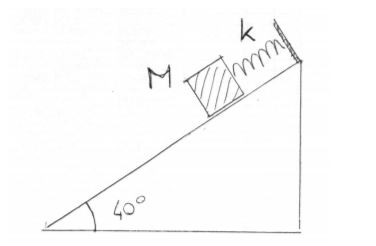
\includegraphics[scale=0.5]{ES2/LUG022016.jpg}
        \end{center}
    \end{figure}
    
    
\begin{figure}[h!]
\textbf{Tema d'Esame di Febbraio 2017}\\ \\
Sapendo che la resistenza $R8$ è attraversata da una corrente $i_8 = 0.20 A$, si calcoli la corrente che attraversa $R3$. Si considerino le seguenti resistenze $R8 = 10 \Omega, R1 = R2 = R3 = 5.0 \Omega , R4 = 12 \Omega , R5 = 15 \Omega $.
	\begin{center}
		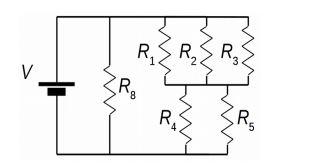
\includegraphics[scale=1.1]{ES5/FEB052017.jpg}
	\end{center}
	\noindent\fbox{
		\parbox{\textwidth}{
			\null\hfill \textbf{Soluzione:} $I_3 = 0.08A$\\
			\textbf{Procedimento: } \\
			Semplificazione delle Resistenze:\\
			$R_{123}=\frac{1}{\frac{1}{R_1}+\frac{1}{R_2}+\frac{1}{R_3}}=\frac{1}{\frac{1}{5\Omega}+\frac{1}{5\Omega}+\frac{1}{5\Omega}}=1.67\Omega$\\ \\ 
			$R_{45}=\frac{R_4\cdot R_5}{R_4 + R_5}=\frac{12\Omega\cdot 15\Omega}{12\Omega + 15\Omega}=6.67\Omega$\\
			$R_{12345}=R_{123}+R_{45}=6.67\Omega+1.67\Omega=8.34\Omega$\\
			Ricordando che la tensione in parallelo non cambia, così come non cambia la corrente in serie:\\
			$V_{tot}=V_{12345}=V_8=R_8\cdot I_8=10\Omega\cdot 0.2A=2V$\\
			$I_{12345}=I_{123}=I_{45}=\frac{V}{R_{12345}}=\frac{2V}{8.34\Omega}=0.24A$\\
			$V_{123}=R_{123}\cdot I_{12345}=1.67\Omega\cdot 0.24A=0.40V$\\
			$I_3=\frac{V_{123}}{R_3}=\frac{0.40V}{5\Omega}=0.08A$
		}
	}	
	
\end{figure}

\begin{figure}[h!]
\textbf{Tema d'Esame di Giugno 2017}\\ \\
 Si determini il valore della resistenza $R_x$ del circuito mostrato nella figura sotto a sinistra. La differenza di potenziale fornita dalla batteria è $3 V$, la corrente $i_3$ che scorre nella resistenza $R_3$ è pari a $0.1 A$ ed i valori delle altre resistenze nel circuito
sono $R1 = R2 = 5 \Omega ,R3 = R4 = 10 \Omega$.
	\begin{center}
		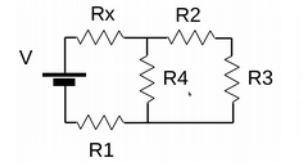
\includegraphics[scale=1.1]{ES5/GIU052017.jpg}
	\end{center}
	\noindent\fbox{
		\parbox{\textwidth}{
			\null\hfill \textbf{Soluzione:} $R_x = 1\Omega$\\
			\textbf{Procedimento: } \\
			Ricordando che la tensione in parallelo non cambia, così come non cambia la corrente in serie proseguiamo semplificando le resistenze e aggiornando man mano corrente e tensione:\\
			
			
			$R_{23}=R_2 + R_3=5\Omega + 10\Omega=15\Omega$\\
			$I_3=I_2=I_{23}=0.1A$\\
			$V_{23}=V_{234}=V_4=R_{23} \cdot I_{23}=15\Omega \cdot 0.1A=1.5V$\\
			$I_{234}=\frac{V_{234}}{R_{234}}=\frac{1.5V}{6\Omega}=0.25A$\\
			$V_1=R_1\cdot I_{234}=5\Omega \cdot 0.25A=1.25V$\\
			$V_x=V_{tot}- V_1 - V_{234}=3V - 1.25V -1.5V=0.25V$\\
			$R_x=\frac{V_x}{I_{234}}=\frac{0.25V}{0.25A}=1\Omega$
		}
	}	
\end{figure}

\begin{figure}[h!]
\textbf{Tema d'Esame di Settembre 2017}\\ \\
Trovare le correnti $i_1, i_2 , i_3$ nei tre rami del circuito qui sotto.
$R1 = 4.0 \Omega, R2 = 6.0 \Omega, R3 = 3.0 \Omega$ ed $ E 1 = 1.5 V,  E 2 = 3.0 V$.
	\begin{center}
		\includegraphics[scale=1.1]{ES5/SET052017.jpg}
	\end{center}
	\noindent\fbox{
		\parbox{\textwidth}{
			\null\hfill \textbf{Soluzione:} $R_x = 1\Omega$\\
			\textbf{Procedimento: } \\
			In questa tipologia di esercizio si deve impostare il sistema per poi trovare le rispettive correnti, per farlo bisogno stabilire arbitrariamente il verso della corrente di ogni maglia.\\
			 Nel nostro caso supporremo che la corrente viaggi in senso orario in entrambe le maglie.\\

			\systeme*{
				I_1=I_2 +I_3,
				\varepsilon_1= R_1\cdot I_1 + R_2\cdot I_2,
				\varepsilon_2= -R_2\cdot I_2 + R_3\cdot I_3
			}
			\\ \\
			Risolvendo il sistema si otterranno i valori delle correnti.\\ \\
			\systeme*{
				I_1=I_2 +I_3,
				1.5= 4\cdot I_1 + 6\cdot I_2,
				3= -6\cdot I_2 + 3\cdot I_3
			}
			\hspace{1.45cm} = \hspace{1.5cm}
			\systeme*{
				I_1=I_2 +I_3,
				1.5= 4\cdot I_2 + 4\cdot I_3 + 6\cdot I_2,
				3= -6\cdot I_2 + 3\cdot I_3
			}\\ \\
			\systeme*{
				I_1=I_2 +I_3,
				1.5= 10\cdot I_2 + 4\cdot I_3,
				I_3=\frac{3V +6\cdot I_2}{3}
			}
			\hspace{1.5cm} = \hspace{1.5cm}
			\systeme*{
				I_1=I_2 +I_3,
				1.5= 10\cdot I_2 + 4\cdot (1 +2\cdot I_2),
				3= -6\cdot I_2 + 3\cdot I_3
			}\\ \\
			\systeme*{
				I_1=I_2 +I_3,
				I_2= -0.139,
				I_3= 1 +2\cdot I_2
			}
			\hspace{2.45cm} = \hspace{1.45cm}
			\systeme*{
				I_1=-0.139 +I_3,
				I_2= -0.139,
				I_3= 0.722
			}\\ \\
			\systeme*{
				I_1= 0.583A,
				I_2= -0.139A,
				I_3= 0.722A
			}\\ \\
		}
	}	
	
\end{figure}
\clearpage
\section{Tipologia Esercizio 6}
\section{Tipologia Esercizio 7}
\section{Tipologia Esercizio 8}

\end{document}
